\section{Zipf-like Distribution}
%introduce zipf's law
%what we did, our methodology
%result graph
Zipf's law has been shown to characterize use of words in a natural language, city populations, 
popularity of website visits and other internet traffic data.

Here we present the first fully consistent empirical study showing that data duplication
pattern in very large scale storage follows Zipf-like distribution. More specifically,
we show that the duplication count of any unique data block is inversely proportional to its rank
in the frequency table, with $\{alpha}$ smaller than unity. 
As far as we know, this is the first study of large scale real user data to disclose
the Zipf-like distribution pattern in data storage area.

\subsection{The model}
Consider a general storage system that holds user's files without any deduplication. 
Let $N$ be the total number of unique data blocks after 
content-defined chunking and deduplication, 
$C_N(i)$ be the number of duplicate copies that the $i$th data block being
stored in storage, given all the unique data blocks be ranked in order of their number of duplicate copies.
Let $S_i$ be the size of $i$th block,
then the actual ranking of the $i$th block is reflected by $\sum_{1}^{i-1}S_i$. 

\subsection{Methodology}
In Aliyun's elastic could service, each VM has several virtual disks: one OS disk and one or more data disks. 
During VM instance creation, the data of OS disk is copied from 
several pre-configured operating system virtual disks depends user's OS choice. 
The data disk is empty at the beginning, user may place their database, website, 
or anything on his data disk, and may attach to more data disks later.

500 users' virtual data disks were scanned using TTTD content-defined chunking, and we performed global perfect deduplication 
to caculate the number of duplicate copies of each individual unique block. We choose 2KB, 4KB, 16KB as the minimum, average
and maximum block size, all variable-sized blocks are compared by their SHA-1 hash arther than real data.

We choose user's data disks rather than OS disks for several reasons: First, the data in OS disks are 
instinctively highly similar, because most of the VM users only make some common or tiny changes to their OSes,
so the data duplication pattern in OS disks cannot reflect the real distribution of general user data.
Second, the data disks are way more important in terms of data safty and backup because they are 
what users really care about.

\subsection{Result}
\begin{figure}
\centering
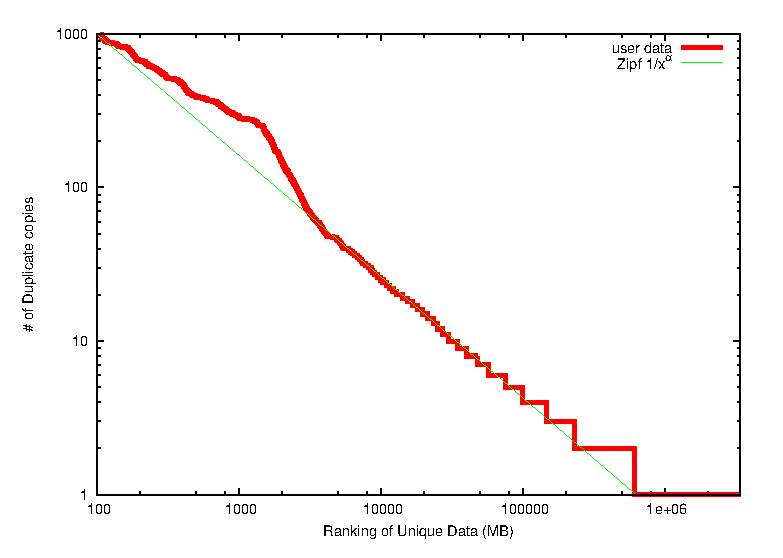
\epsfig{file=images/log-log.disk.eps, height=2in, width=2.66in}
\caption{# of duplicate copies vesus block ranking}
\label{figure:zipf}
\end{figure}